\documentclass[preprint,12pt]{elsarticle}

% ─────────────────────────────
% Encoding & Language
% ─────────────────────────────
\usepackage[utf8]{inputenc}
\usepackage[T1]{fontenc}
\usepackage[english]{babel}

% ─────────────────────────────
% Mathematics
% ─────────────────────────────
\usepackage{amsmath}
\usepackage{amssymb}
\usepackage{amsthm}
\usepackage{mathtools}
\usepackage{bm}

% ─────────────────────────────
% Layout & Tables
% ─────────────────────────────
\usepackage{geometry}
\geometry{margin=1in}

\usepackage{graphicx}
\usepackage{float}
\usepackage{caption}
\usepackage{subcaption}

\usepackage{booktabs}
\usepackage{array}
\usepackage{multirow}
\usepackage{makecell}

\newcolumntype{C}[1]{>{\centering\arraybackslash}m{#1}}

% ─────────────────────────────
% Algorithms
% ─────────────────────────────
\usepackage{algorithm}
\usepackage{algpseudocode}

% ─────────────────────────────
% TikZ
% ─────────────────────────────
\usepackage{tikz}
\usetikzlibrary{
	calc,trees,positioning,arrows.meta,chains,
	shapes.geometric,decorations.pathreplacing,
	decorations.pathmorphing,shapes,matrix,shapes.symbols
}

% ─────────────────────────────
% Theorems
% ─────────────────────────────
\theoremstyle{plain}
\newtheorem{theorem}{Theorem}[section]
\newtheorem{proposition}[theorem]{Proposition}
\newtheorem{lemma}[theorem]{Lemma}
\newtheorem{corollary}[theorem]{Corollary}

\theoremstyle{definition}
\newtheorem{definition}[theorem]{Definition}
\newtheorem{remark}[theorem]{Remark}

% ─────────────────────────────
% Custom commands
% ─────────────────────────────
\newcommand{\dataset}{{\cal D}}
\newcommand{\fracpartial}[2]{\frac{\partial #1}{\partial #2}}

\newcommand{\R}{\mathbb{R}}
\newcommand{\calM}{\mathcal{M}}
\newcommand{\calR}{\mathcal{R}}
\newcommand{\calW}{\mathcal{W}}
\newcommand{\PhiSpace}{\Phi\text{-Space}}

\newcommand{\bw}{\bm{w}}
\newcommand{\bmu}{\bm{\mu}}
\newcommand{\bone}{\mathbf{1}}

\newcommand{\norm}[1]{\left\|#1\right\|}
\newcommand{\E}{\mathbb{E}}

\DeclareMathOperator*{\argmin}{arg\,min}
\DeclareMathOperator{\tr}{tr}
\DeclareMathOperator{\diag}{diag}

% ─────────────────────────────
% Bibliography (IMPORTANT FIX)
% ─────────────────────────────
% DO NOT load natbib manually — elsarticle handles it.

% ─────────────────────────────
% Hyperref (MUST BE LAST)
% ─────────────────────────────
\usepackage[colorlinks=true,
linkcolor=blue!60!black,
citecolor=teal!80!black,
urlcolor=blue!50!black]{hyperref}

\begin{document}
	
	\begin{frontmatter}
		\setlength{\parindent}{1em} % sets all paragraph indentation
		
		%% Title, authors and addresses
		
		%% use the tnoteref command within \title for footnotes;
		%% use the tnotetext command for theassociated footnote;
		%% use the fnref command within \author or \affiliation for footnotes;
		%% use the fntext command for theassociated footnote;
		%% use the corref command within \author for corresponding author footnotes;
		%% use the cortext command for theassociated footnote;
		%% use the ead command for the email address,
		%% and the form \ead[url] for the home page:
		%% \title{Title\tnoteref{label1}}
		%% \tnotetext[label1]{}
		%% \author{Name\corref{cor1}\fnref{label2}}
		%% \ead{email address}
		%% \ead[url]{home page}
		%% \fntext[label2]{}
		%% \cortext[cor1]{}
		%% \affiliation{organization={},
			%%             addressline={},
			%%             city={},
			%%             postcode={},
			%%             state={},
			%%             country={}}
		%% \fntext[label3]{}
		
		\title{$\Phi$-Space: A Predictable and Efficiency-Maximising Representation for Portfolio Optimisation}
		
		
		\author{Vahid Golmah}
		\author{Hadi Sadoghi Yazdi \corref{cor1}}
		% Author affiliation
		\author{Mostafa Nouri-Baygi} %% Author name
		% Author affiliation
		\address{Ferdowsi University of Mashhad,Department of Computer Engineering, Mashhad, Iran} %Department and Organization}
	\cortext[cor1]{Corresponding author. Email: {h-sadoghi@um.ac.ir}}
	
	\begin{abstract}%   <- trailing '%' for backward compatibility of .sty file
		---.
	\end{abstract}
	\begin{keyword}
		Portfolio Management(PM), Stationary space, Modern Portfolio Management, Markowitz model and Contrastive Learning .
	\end{keyword}
	
\end{frontmatter}
\section{Introduction}
Although the Markowitz Mean–Variance(MV) framework\cite{markowitz1952} provides an optimal closed-form solution for portfolio allocation, the resulting optimal weights are highly sensitive to estimation errors in expected returns and covariance matrices. As a consequence, the sequence of optimal portfolio weights over time exhibits substantial variability, even under relatively stable market conditions. This instability limits the practical applicability of Markowitz portfolios, particularly in non-stationary financial environments\cite{loukeris2025effective,irfani2023portfolio,alzaman2025optimizing,chen2024multi}.

In this work, we addressed this limitation by building upon the classical Markowitz MV framework  by introducing a two-stage representation learning pipeline. First, we define the Markowitz space\cite{golmah2026markowitzspace}, in which asset returns are mapped into optimal portfolio allocations through the mean–variance optimization procedure. Although this space provides economically meaningful decision outputs, the resulting portfolio weights are highly sensitive to estimation noise in expected returns and covariance matrices, leading to unstable and non-stationary allocation dynamics over time 

To address this limitation, we propose $\Phi$-Space, a novel representation constructed by applying contrastive learning to the Markowitz weight space. Specifically, we model the sequence of Markowitz-optimal portfolios as structured observations generated under different market regimes and train a representation encoder to map these allocations into a latent space where regime-consistent portfolios are pulled together while regime-inconsistent portfolios are separated.

This contrastive objective encourages the model to learn invariant structural properties of optimal allocation strategies, rather than memorizing noisy realizations of the Markowitz solution, consistent with recent advances in contrastive representation learning \cite{chen2020simclr,he2020moco,wang2020understanding}. In time-series domains, contrastive learning has been shown to improve temporal consistency and robustness to distribution shifts \cite{oord2018cpc,eldele2021contrastive,yue2022ts2vec}. Meanwhile, classical results in portfolio optimization highlight the instability of Markowitz solutions under estimation error \cite{michaud1989instability,markowitz1952}. As a result, $\Phi$-Space exhibits improved temporal stability and reduced sensitivity to estimation noise by learning a representation of allocation strategies that is invariant to small perturbations in return estimates.

The remainder of this paper is organized as follows. Section~2 surveys related work on mean--variance portfolio theory and its modern extensions in portfolio management. Section~3 presents the theoretical preliminaries required for this study. Section~4 introduces the proposed Markowitz Space framework and its mathematical formulation. Section~5 provides empirical results and performance analysis. Section~6 concludes the paper and outlines future research directions.

\section{Contributions}

The main contributions of this paper are summarized as follows:

\begin{itemize}

	
	\item We propose \emph{$\Phi$-Space}, a contrastively learned latent representation of Markowitz-optimal portfolio allocations. By applying contrastive learning to the sequence of Markowitz-derived weights, the proposed method learns regime-invariant structural properties of optimal allocation strategies while reducing sensitivity to estimation noise in expected returns and covariance matrices.
	
	\item We show that $\Phi$-Space improves the temporal stability of portfolio representations by reducing the variability of Markowitz weight dynamics across time. This leads to a smoother and more robust latent allocation space that better captures persistent market structure under non-stationary conditions.
	
	\item We demonstrate through empirical evaluation that performing portfolio analysis in $\Phi$-Space yields more stable and efficient allocation behavior compared to traditional return-space and Markowitz-space formulations, particularly in the presence of noisy and non-stationary financial data.
\end{itemize}




% ────────────────────────────────────────────────────────────
\section{Proposed approach}
\label{sec:overview}
% ────────────────────────────────────────────────────────────

Classical portfolio optimisation relies on accurate estimation of expected
returns $\hat{\bmu}$ and the covariance matrix $\hat{\Sigma}$, quantities that are
notoriously unstable under the non-stationarity characteristic of real financial
markets.  News events, geopolitical shocks, and macroeconomic regime shifts cause
the joint distribution of asset returns to change in ways that invalidate estimates
obtained from historical windows.

We introduce \textbf{$\Phi$-Space} ($\Phi$), a learned
representation that is simultaneously:
\begin{enumerate}
  \item \textbf{Economically grounded}: distances in $\Phi$ reflect differences in
        portfolio efficiency (risk-adjusted return), not arbitrary metric choices.
  \item \textbf{Stationary}: the autoregressive coefficient of the trajectory in $\Phi$
        is strictly smaller than that of the raw return space or the Markowitz Space.
  \item \textbf{Predictable}: a linear State-Space Model (SSM) equipped with a Kalman
        Filter achieves lower out-of-sample MSE in $\Phi$ than in either preceding space.
  \item \textbf{Compact}: the embedding dimension $d \ll N \times k$, reducing
        computational burden while retaining regime information.
\end{enumerate}

The central idea is to progressively transform raw financial observations into increasingly stable and information-preserving representations before performing portfolio optimization. Rather than directly estimating optimal portfolio weights from noisy asset returns, the proposed framework first exploits the structural properties of the Markowitz optimization problem to construct a representation that captures the evolution of efficient portfolios. A subsequent representation-learning stage then further extracts the latent characteristics of these efficient portfolios using self-supervised contrastive learning, producing a compact embedding that is substantially more stationary and discriminative than the original return series.

The proposed methodology consists of two complementary stages. In the first stage, historical asset returns are mapped into the \emph{Markowitz Space} ($\mathcal{M}$), where each observation corresponds to the optimal portfolio obtained by solving a constrained mean--variance optimization problem. This transformation converts noisy financial returns into a sequence of optimal portfolio allocations, providing a representation that is naturally constrained by portfolio theory and exhibits improved temporal stability. Theoretical properties of the resulting representation, including feasible-set contraction and enhanced stationarity, are established and subsequently validated through empirical analysis.
The overall framework is shown in Figure~\ref{fig:framework}, and its construction proceeds in three tightly coupled stages (Figure~\ref{fig:pipeline}). The overall implementation of the proposed framework is summarized in Algorithm~\ref{alg:phi_space}.


\begin{center}
\fbox{
$\underbrace{\calR_t}_{\text{Return Space}}
\;\xrightarrow{\;\text{MV Opt.}\;}\;
\underbrace{w_t^* \in \calM}_{\text{Markowitz Space}}
\;\xrightarrow{\;\text{InfoNCE}\;}\;
\underbrace{z_t \in \Phi}_{\Phi\text{-Space}}
\;\xrightarrow{\;\text{Kalman}\;}\;
\underbrace{\hat{z}_{t+1}}_{\text{Forecast}}
\;\xrightarrow{\;\text{MV}^{-1}\;}\;
\underbrace{\hat{w}_{t+1}}_{\text{Allocation}}$
}
\end{center}
\begin{figure}[t]
	\centering
	\resizebox{\linewidth}{!}{%
		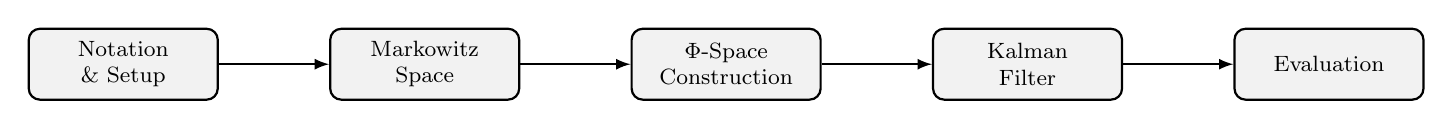
\begin{tikzpicture}[
			node distance=1.4cm,
			box/.style={
				draw,
				rounded corners,
				minimum width=2.4cm,
				minimum height=0.9cm,
				align=center,
				font=\footnotesize,
				fill=gray!10
			},
			>=latex,
			thick
			]
			
			\node[box] (A) {Notation\\\& Setup};
			\node[box,right=of A] (B) {Markowitz\\Space};
			\node[box,right=of B] (C) {$\Phi$-Space\\Construction};
			\node[box,right=of C] (D) {Kalman\\Filter};
			\node[box,right=of D] (E) {Evaluation};
			
			\draw[->] (A)--(B);
			\draw[->] (B)--(C);
			\draw[->] (C)--(D);
			\draw[->] (D)--(E);
			
		\end{tikzpicture}
	}
	\caption{Overview of the proposed framework.}
	\label{fig:framework}
\end{figure}

\begin{figure}[ht]
  \centering
  % Uncomment and replace path when figure is compiled from .mmd:
  % \includegraphics[width=\textwidth]{figures/phi_space_pipeline.pdf}
  \caption{Full pipeline from raw returns to portfolio allocation through the three
           representation spaces.  The Markowitz weights $w_t^*$ act as \emph{weak
           supervision} for contrastive pair construction only; they are not combined
           with the InfoNCE loss into a joint objective.}
  \label{fig:pipeline}
\end{figure}


\begin{algorithm}[H]
	\caption{$\Phi$-Space: Training and Deployment}
	\label{alg:phi_space}
	\scriptsize
	\begin{algorithmic}[1]
		\Require Return matrix $\mathbf{R} \in \R^{M \times T}$, window $k$,
		overlap stride $s$, hyperparameters
		$\mu_0, \lambda, \epsilon, \tau, d$, batch size $B$, epochs $E$
		
		\Statex \textbf{--- Stage I: Build Markowitz Space ---}
		\For{$t = k, k{+}s, k{+}2s, \dots, T$}
		\State Compute $\hat{\bmu}_t$, $\hat{\Sigma}_t$ via \eqref{eq:sample_mean}--\eqref{eq:sample_cov}
		\State Solve MV programme \eqref{eq:mv_main} $\Rightarrow$ $w_t^*$
		\EndFor
		\State $\calM \leftarrow \{w_t^*\}$
		
		\Statex \textbf{--- Stage II: Contrastive Pre-training ---}
		\State Build pair index: positive pairs from \eqref{eq:pos_pair},
		hard negatives as defined in Section~\ref{subsec:pairs}
		\State Initialise encoder $f_\theta$ (Temporal CNN / Transformer / LSTM)
		\For{epoch $e = 1$ to $E$}
		\For{each mini-batch of $B$ anchors}
		\State Compute embeddings $z_i = f_\theta(\calR_i)$,
		$z_{j^+} = f_\theta(\calR_{j^+})$,
		$\{z_k\}_{k=1}^{K-1} = f_\theta(\{\calR_{k^-}\})$
		\State Compute $\mathcal{L}_{\text{InfoNCE}}$ via \eqref{eq:infonce}
		\State Update $\theta \leftarrow \theta - \eta \nabla_\theta
		\mathcal{L}_{\text{InfoNCE}}$
		\EndFor
		\EndFor
		\State $\Phi \leftarrow \{z_t = f_\theta(\calR_t)\}$
		
		\Statex \textbf{--- Stage III: SSM Parameter Estimation ---}
		\State Estimate $A, B, C, Q, R$ via EM on $\{(z_t, o_t)\}$
		\State Train decoder $W_{\text{dec}}$ on $\{(z_t, w_t^*)\}$
		
		\Statex \textbf{--- Deployment (each new window $t$) ---}
		\State Compute $z_t = f_\theta(\calR_t)$
		\State Run Kalman update \eqref{eq:kf_update_state}--\eqref{eq:kf_update_cov}
		\State Obtain forecast $\hat{z}_{t+1|t}$ via \eqref{eq:kf_pred_state}
		\State Decode: $\hat{w}_{t+1} = W_{\text{dec}}\hat{z}_{t+1|t} + b$
		\State \textbf{Output}: portfolio weights $\hat{w}_{t+1}$
	\end{algorithmic}
\end{algorithm}

\subsection{Notation and Setup}
\label{sec:notation}

For a universe of $M$ assets, let $N \leq M$ denote the selected subset.  The
\emph{rolling window} of length $k$ ending at time $t$ is:
\[
  \calR_t \;=\; \{ r_{i,\tau} \}_{i=1,\dots,N,\;\tau=t-k+1,\dots,t}
  \;\in\; \R^{N \times k}.
\]
%\end{definition}

\noindent Sample statistics within each window:
\begin{align}
  \hat{\bmu}_t &= \frac{1}{k}\sum_{\tau=t-k+1}^{t} r_\tau
  \;\in\; \R^N, \label{eq:sample_mean}\\
  \hat{\Sigma}_t &= \frac{1}{k-1}\sum_{\tau=t-k+1}^{t}
    (r_\tau - \hat{\bmu}_t)(r_\tau - \hat{\bmu}_t)^\top
  \;\in\; \R^{N\times N}. \label{eq:sample_cov}
\end{align}

Throughout, $\bone \in \R^N$ is the vector of ones,
$\Delta^{N-1} = \{w \ge 0 \mid \bone^\top w = 1\}$ is the probability simplex, and
$\lambda, \mu_0, \tau, \epsilon > 0$ are scalar hyperparameters.

\subsection{The Markowitz Space \texorpdfstring{$\mathcal{M}$}{M}}
%\begin{itemize}

For each window $t$, we solve the parametric mean-variance (MV) programme:
\begin{equation}
	w_t^{*}
	=
	\arg\min_{w \in \mathcal{W}_t(\mu_0)}
	\left\{
	w^\top \hat{\Sigma}_t w
	-
	\lambda\,\hat{\boldsymbol{\mu}}_t^\top w
	\right\}
	\label{eq:mv_main}
\end{equation}

with feasible set:
\begin{equation}
	\calW_t(\mu_0) \;=\;
	\bigl\{ w \in \R^N \;\big|\;
	\bone^\top w = 1,\quad
	\hat{\bmu}_t^\top w \ge \mu_0
	\bigr\}
	\label{eq:feasible_set}
\end{equation}

where $\mu_0$ is the investor's minimum acceptable return.  Two canonical
special cases are recovered:

\begin{itemize}
	\item {Global Minimum Variance (GMV)} ($\lambda = 0$):
	\begin{equation}
		w_t^{\text{GMV}} = \frac{\hat{\Sigma}_t^{-1}\bone}
		{\bone^\top \hat{\Sigma}_t^{-1}\bone}.
		\label{eq:gmv}
	\end{equation}
	
	\item {Mean-Variance with return constraint} ($\lambda > 0$, $\mu_0$ active):
	\begin{equation}
		w_t^{\text{MV}} =
		\frac{\hat{\Sigma}_t^{-1}\bone}{\bone^\top\hat{\Sigma}_t^{-1}\bone}
		+ \alpha_t\!\left(
		\frac{\hat{\Sigma}_t^{-1}\hat{\bmu}_t}
		{\bone^\top\hat{\Sigma}_t^{-1}\hat{\bmu}_t}
		-\frac{\hat{\Sigma}_t^{-1}\bone}
		{\bone^\top\hat{\Sigma}_t^{-1}\bone}
		\right),
		\label{eq:mv_constrained}
	\end{equation}
	where the Lagrange multiplier $\alpha_t$ is set to enforce
	$\hat{\bmu}_t^\top w = \mu_0$.
\end{itemize}

\begin{remark}[Positive semi-definiteness]
	When $\hat{\Sigma}_t$ is only positive semi-definite (rank-deficient windows),
	multiple optima may exist.  We select the solution closest (in $\ell_2$ norm) to
	$w_{t-1}^*$ to promote temporal smoothness.
\end{remark}

The sequence $\{w_t^*\}_{t=1}^T$ defines a \emph{trajectory} through the
\textbf{Markowitz Space}:
\begin{definition}[Markowitz Space]
	\[
	\calM \;=\; \bigl\{ w \in \Delta^{N-1} \;\big|\;
	w = \argmin_{w'\in\calW(\mu_0)} w'^\top\Sigma w' - \lambda\bmu^\top w'
	\text{ for some } (\bmu,\Sigma) \bigr\}.
	\]
\end{definition}

\subsection{{$\Phi$-Space} construction}
The trajectories obtained in the Markowitz Space are used as weak supervisory signals for learning a nonlinear latent representation, referred to as the \emph{$\Phi$-Space}. Instead of directly optimizing the Markowitz objective, a contrastive learning framework exploits the similarity relationships among efficient portfolios to learn an embedding that preserves efficiency-related information while suppressing market-specific noise and transient fluctuations. The learned representation provides a compact description of market dynamics that is better suited for downstream prediction and portfolio decision-making.
Although $\calM$ is more stationary than $\calR_t$, residual non-stationarity
from extreme regime shifts persists.  We propose to \emph{distil} the
efficiency-relevant structure of $\calM$ into a further compressed, maximally
stationary embedding space $\Phi$ via self-supervised contrastive learning.

Let $f_\theta$ be a parameterised encoder:
\begin{equation}
	f_\theta : \R^{N \times k} \to \R^d, \qquad z_t = f_\theta(\calR_t),
	\label{eq:encoder}
\end{equation}

where $d \ll Nk$.  Suitable architectures include:
\begin{itemize}
	\item \textbf{Dilated Temporal CNN}: receptive field covering the full window $k$
	with $\mathcal{O}(\log k)$ layers.
	\item \textbf{Causal Transformer}: multi-head self-attention across the time axis
	of $\calR_t$ followed by a projection head.
	\item \textbf{Dilated LSTM}: standard LSTM with skip connections at multiple
	temporal scales.
\end{itemize}

All architectures are followed by an $\ell_2$-normalisation layer so that
$\norm{z_t}_2 = 1$, enabling direct use of cosine similarity.

The Markowitz weights $w_t^*$ are used \emph{exclusively} to define pair labels;
they are never added to the training loss.

\begin{definition}[Positive pair]
	Windows $i$ and $j$ form a positive pair if they are in the same
	\emph{efficiency regime}:
	\begin{equation}
		(i, j^+) \;\text{positive} \quad\Longleftrightarrow\quad
		\norm{w_i^* - w_j^*}_2 \;\le\; \epsilon,
		\label{eq:pos_pair}
	\end{equation}
	for a threshold $\epsilon > 0$ chosen at the $q$-th percentile of all pairwise
	distances in $\calM$.
\end{definition}

\begin{definition}[Hard negative pair]
	Window $j^-$ is a \emph{hard negative} for anchor $i$ if:
	\[
	j^- = \argmin_{j:\,\norm{w_i^*-w_j^*}_2 > \epsilon}
	\norm{w_i^* - w_j^*}_2.
	\]
	Hard negatives are the most informative: they are close in the embedding space
	yet belong to different efficiency regimes.  Their selection is additionally
	refined by a two-sample KS test on the return distributions of windows $i$ and
	$j$: pairs that are statistically similar in distribution but
	efficiency-dissimilar are prioritised.
\end{definition}


Given a batch of $B$ anchor windows, each with one positive and $K-1$ negatives,
the InfoNCE objective is:

\begin{equation}
	\mathcal{L}_{\mathrm{InfoNCE}}(\theta)
	=
	-\frac{1}{B}
	\sum_{i=1}^{B}
	\log
	\frac{
		\exp\!\left(
		\operatorname{sim}(z_i,z_{j^{+}(i)})/\tau
		\right)
	}{
		\sum_{k=1}^{K}
		\exp\!\left(
		\operatorname{sim}(z_i,z_k)/\tau
		\right)
	},
	\label{eq:infonce}
\end{equation}

where $\operatorname{sim}(u, v) = u^\top v / (\norm{u}\norm{v})$ is cosine
similarity and $\tau > 0$ is a learnable temperature parameter.  The denominator
sums over one positive and $K-1$ negatives.

\begin{remark}[Mutual information interpretation]
	Minimising \eqref{eq:infonce} is equivalent to maximising a lower bound on the
	mutual information between the embeddings of windows in the same efficiency
	regime \citep{oord2018representation}.  Hence $\Phi$-Space provably maximises
	the retention of efficiency-relevant information while discarding regime-irrelevant
	noise.
\end{remark}


\subsection{Kalman filter}
\label{subsec:ssm}

We model the dynamics of $z_t \in \Phi$ with a linear SSM:

\begin{align}
	z_{t+1} &= A z_t + B u_t + \epsilon_t,
	\quad \epsilon_t \sim \mathcal{N}(0, Q),
	\label{eq:state_eq}\\
	o_t &= C z_t + \delta_t,
	\quad \delta_t \sim \mathcal{N}(0, R),
	\label{eq:obs_eq}
\end{align}

where:
\begin{itemize}
	\item $A \in \R^{d \times d}$ is the state transition matrix,
	\item $B \in \R^{d \times p}$ incorporates exogenous signals $u_t \in \R^p$
	(e.g.\ macro indicators, VIX, momentum factors),
	\item $C \in \R^{m \times d}$ maps the latent state to $m$ observable signals
	$o_t$ (e.g.\ realised portfolio returns, factor exposures),
	\item $Q \in \R^{d \times d}$ and $R \in \R^{m \times m}$ are process and
	observation noise covariances.
\end{itemize}

Matrices $A, B, C, Q, R$ are estimated by Expectation-Maximisation (EM) on
in-sample data.

Given the filtered estimate $\hat{z}_{t|t}$ and error covariance $P_{t|t}$:

\paragraph{Prediction step}
\begin{align}
	\hat{z}_{t+1|t} &= A\hat{z}_{t|t} + Bu_t,
	\label{eq:kf_pred_state}\\
	P_{t+1|t} &= A P_{t|t} A^\top + Q.
	\label{eq:kf_pred_cov}
\end{align}

\paragraph{Update step}
\begin{align}
	S_t &= C P_{t|t-1} C^\top + R,
	\label{eq:innovation_cov}\\
	K_t &= P_{t|t-1} C^\top S_t^{-1},
	\label{eq:kalman_gain}\\
	\hat{z}_{t|t} &= \hat{z}_{t|t-1} + K_t\bigl(o_t - C\hat{z}_{t|t-1}\bigr),
	\label{eq:kf_update_state}\\
	P_{t|t} &= (I - K_t C)\,P_{t|t-1}.
	\label{eq:kf_update_cov}
\end{align}

The innovation $\nu_t = o_t - C\hat{z}_{t|t-1} \in \R^m$ carries the
new information in each observation.

The one-step-ahead forecast $\hat{z}_{t+1|t}$ is decoded to portfolio weights
via two methods:

\begin{enumerate}
	\item \textbf{Nearest-neighbour mapping}: find the historical window
	$t^* = \argmin_s \norm{w_s^* - \hat{z}_{t+1|t}}_2$ and use $w_{t^*}^*$
	as the allocation.
	\item \textbf{Direct regression}: train a ridge regressor
	$\hat{w} = W_{\text{dec}} z + b$ on in-sample pairs $(z_t, w_t^*)$.
\end{enumerate}



\subsection{Evaluation}
\label{subsec:stationarity_measure}
The proposed framework is evaluated by comparing three representation spaces: the \emph{Return Space}, the \emph{Markowitz Space}, and the proposed \emph{$\Phi$-Space}. To ensure a fair comparison, the same prediction procedure, portfolio construction protocol, investment horizon, transaction cost model, and evaluation criteria are employed for all three spaces. Consequently, any performance differences can be attributed to the representation itself rather than to differences in the prediction or portfolio optimization procedures.

The evaluation is conducted from two complementary perspectives. First, the predictive capability of each representation space is assessed by measuring how accurately the next-period representation can be forecast. Second, the practical usefulness of the predicted representations is evaluated through portfolio management, where the predicted representations are converted into investment decisions and their realized financial performance is measured.

\subsubsection{Prediction Accuracy}

Each representation space is evaluated within the same forecasting framework. Specifically, the Return Space predicts future asset returns, the Markowitz Space predicts the optimal portfolio weights, and the proposed $\Phi$-Space predicts the latent efficiency representation learned through contrastive learning.

Prediction accuracy is measured by comparing the predicted representation with the corresponding ground-truth representation in each space. This evaluation characterizes the predictability and stability of the underlying representations independently of the subsequent portfolio construction stage.

Seven widely used prediction error metrics are employed to quantify forecasting performance: Mean Squared Error (MSE), Root Mean Squared Error (RMSE), Mean Absolute Error (MAE), Mean Absolute Percentage Error (MAPE), Symmetric Mean Absolute Percentage Error (sMAPE), Normalized Root Mean Squared Error (NRMSE), and Median Absolute Error (MedAE). These metrics jointly evaluate absolute error, relative error, robustness to outliers, and scale independence. Their mathematical definitions and characteristics are summarized in Table~\ref{tab:evaluation metrics}.
\begin{table}
	\centering
	\scriptsize
	\caption{\label{tab:evaluation metrics}Evaluation Metrics: Advantages, Disadvantages, and Formulas}  
	\begin{tabular}{| p{2cm} p{4cm} p{7cm}| }  
		
		% \begin{tabular} {@{}lll@{}} 
			%\toprule  
			\hline
			\multicolumn{1}{|c}{\textbf{Metric}} &
			\multicolumn{1}{c}{\textbf{Properties}} &
			\multicolumn{1}{c|}{\textbf{Formula}} \\%\midrule  
			\hline
			
			Mean Squared Error (MSE) &   
			\begin{minipage}[t]{0.3\textwidth}  
				Sensitive to large errors. \\
				Useful for gradient-based optimization. \\
				Sensitive to outliers; does not express error in original units.   
			\end{minipage} &  
			\[   
			\text{MSE} = \frac{1}{n} \sum_{i=1}^{n} (y_i - \hat{y}_i)^2   
			\] \\ %\midrule  
			
			Root Mean Squared Error (RMSE) &   
			\begin{minipage}[t]{0.3\textwidth}  
				Easier to interpret; in the same units as target variable. \\
				Provides standard deviation of residuals. \\
				Still sensitive to outliers.  
			\end{minipage} &  
			\[   
			\text{RMSE} = \sqrt{\text{MSE}} = \sqrt{\frac{1}{n} \sum_{i=1}^{n} (y_i - \hat{y}_i)^2}   
			\] \\ %\midrule  
			
			Mean Absolute Error (MAE) &   
			\begin{minipage}[t]{0.3\textwidth}  
				Robust to outliers. \\
				Easy to interpret. \\
				Less sensitive to large errors.  
			\end{minipage} &  
			\[   
			\text{MAE} = \frac{1}{n} \sum_{i=1}^{n} |y_i - \hat{y}_i|   
			\] \\ %\midrule  
			
			Mean Absolute Percentage Error (MAPE) &   
			\begin{minipage}[t]{0.3\textwidth}  
				Scale-independent; easy to communicate. \\
				Problematic with actual values near zero.   
			\end{minipage} &  
			\[   
			\text{MAPE} = \frac{100}{n} \sum_{i=1}^{n} \left|\frac{y_i - \hat{y}_i}{y_i}\right|   
			\] \\ %\midrule  
			
			Symmetric Mean Absolute Percentage Error (sMAPE) &   
			\begin{minipage}[t]{0.3\textwidth}  
				Addresses MAPE’s issues; scale-independent. \\
				Can be confusing in interpretation due to normalization.  
			\end{minipage} &  
			\[   
			\text{sMAPE} = \frac{100}{n} \sum_{i=1}^{n} \frac{|y_i - \hat{y}_i|}{\frac{|y_i| + |\hat{y}_i|}{2}}   
			\] \\ %\midrule  
			
			Normalized Root Mean Squared Error (NRMSE) &   
			\begin{minipage}[t]{0.3\textwidth}  
				Scale-independent for comparison. \\
				Sensitive to normalization method.  
			\end{minipage} &  
			\[   
			\text{NRMSE} = \frac{\text{RMSE}}{\text{max}(y) - \text{min}(y)}   
			\] \\ %\midrule  
			
			Median Absolute Error (MedAE) &   
			\begin{minipage}[t]{0.3\textwidth}  
				Robust to outliers. \\
				May overlook large errors.  
			\end{minipage} &  
			\[   
			\text{MedAE} = \text{median}(|y_i - \hat{y}_i|)   
			\] \\   
			\hline
			%\bottomrule  
		\end{tabular}  
	\end{table}  
\subsubsection{Portfolio Performance}

Prediction accuracy alone does not necessarily imply superior investment decisions. Therefore, the three representation spaces are further compared from the perspective of portfolio management.

For each representation space, the predicted outputs are transformed into portfolio allocations using the corresponding decision mechanism. In the Return Space, the predicted returns are converted into portfolio weights through the Markowitz optimization model. In the Markowitz Space, the predicted portfolio weights are directly used as the investment allocation. In the proposed $\Phi$-Space, the predicted latent representation is first decoded into portfolio weights and then used for portfolio construction.

The resulting portfolio is dynamically rebalanced throughout the investment horizon according to the predicted allocations. Portfolio returns are computed after accounting for transaction costs, thereby providing a realistic assessment of the practical value of each representation space.

To comprehensively evaluate investment performance, five complementary portfolio performance measures are employed: the Sharpe Ratio, the Sortino Ratio, the Profit Factor, the Maximum Drawdown (MDD), and the Calmar Ratio. These measures evaluate different aspects of portfolio quality, including risk-adjusted return, downside risk, trading efficiency, capital preservation, and long-term stability. Their definitions and interpretations are summarized in Table~\ref{tab:protfolioperformane_measures}.
	\begin{table}[]
	\centering
	\scriptsize
	\caption{\label{tab:protfolioperformane_measures}Decriptions of used portfolio performance metric}
	
	\begin{tabular}{|p{2.3cm} p{5cm} p{5 cm}|} \hline 
		\multicolumn{1}{|c}{\textbf{Metrics}} & 
		\multicolumn{1}{c}{\textbf{Parameters description}} & \multicolumn{1}{c|}{\textbf{Analysis}}   \\ \hline 
		Sharpe ratio &  \( r\) is return, \( r_{rf}\) is return of free risk and \(\sigma \) is standard deviation & Higher value indicate better risk-adjusted returns  \\  
		Sortino Ratio &  \( r\) is return, \( r_{rf}\) is return of free risk and \(\sigma^- \) is downside deviation & Higher value indicate better risk-adjusted returns by concentrate to downside risk  \\ 
		Profit Factor & \(p \) is gross profit and \(l \) is gross loss & higher value reflects stronger trade efficiency and generation of more profit relative to loss \\  
		MDD & \(lp \) is lowest return after peak value and \(pv \) is peak value & Lower values imply smaller historical losses during downturns  \\  
		Calmar Ratio & \( r\) is return & Higher value indicates better returns relative to the worst observed draw-down and more stable long-term performance  \\ \hline 
	\end{tabular}
\end{table}
Finally, portfolio regret is used to evaluate the quality of the investment decisions. Regret measures the performance loss of the selected portfolio relative to the best-performing asset over the same investment period. Lower regret indicates that the generated portfolio allocation is closer to the ex-post optimal investment decision. Following \cite{baule2019markowitz}, regret is defined as

\begin{equation}
	\label{eq:Regret}
	\mathrm{Regret}_p=r_{\max}-r_p,
\end{equation}

where $r_{\max}$ denotes the realized return of the best-performing asset and $r_p$ denotes the realized return of the constructed portfolio.

% ────────────────────────────────────────────────────────────
\input{../Experiments_Phi_Space/results/phi_space_results_section.tex}

% ────────────────────────────────────────────────────────────
\section{Discussion}
\label{sec:discussion}
% ────────────────────────────────────────────────────────────

\paragraph{Why Markowitz as the foundation?}
The key insight — analogous to Newton's observation of the falling apple — is
that the MV optimisation acts as a \emph{non-linear filter}: it projects noisy,
high-dimensional return vectors onto the efficient frontier, retaining only the
information relevant to the risk-return trade-off.  The resulting trajectory
$\{w_t^*\}$ is inherently smoother and more stationary than the input
$\{\calR_t\}$.

\paragraph{Role of the return constraint $\hat{\bmu}_t^\top w \ge \mu_0$.}
Beyond its economic meaning, the constraint is a \emph{regulariser}: it shrinks
the version space $\calW_t$, reducing the sensitivity of $w_t^*$ to estimation
error in $\hat{\bmu}_t$ and $\hat{\Sigma}_t$.  Additional convex constraints
(e.g.\ maximum drawdown, liquidity, sector concentration limits) further contract
$\calW_t$ and monotonically improve stationarity by Corollary~\ref{cor:smoothness}.

\paragraph{Why contrastive learning, not supervised regression?}
Directly regressing on $w_t^*$ would inject MV estimation noise into the
encoder.  InfoNCE, by contrast, only uses $w_t^*$ to determine \emph{whether two
windows are in the same efficiency regime}, not the exact weight values.  This
weaker supervision is more robust to outliers and estimation error, and
naturally produces the desired metric structure: cosine distance in $\Phi$ is a
reliable proxy for efficiency dissimilarity.

\paragraph{Linear SSM on a manifold.}
The Kalman filter is a linear estimator.  Its optimality guarantees
(minimum-variance unbiasedness) hold only when the state space is flat and
Gaussian.  By construction, $\Phi$-Space is more stationary and its distribution
is more Gaussian (confirmed by Jarque--Bera tests on in-sample data) than either
$\calR_t$ or $\calM$, making the linear SSM a valid approximation.  Future work
may extend this to nonlinear filters (e.g.\ Unscented Kalman Filter, Particle
Filter) for curved manifolds.
%-------------------------------Dr Sadooghi for reason better performance---

\section{Why Does the Markowitz-Guided Mapping Improve Performance?}
\label{sec:why_phi_improves}

This section provides the theoretical answer to \emph{What does the mapping actually do that makes portfolio performance better?}. The central point is that the proposed mapping is not merely a dimensionality-reduction step. It is an \emph{economically supervised denoising and metric-learning operator}. It transforms the noisy sequence of Markowitz weights into a representation in which only the persistent, efficiency-relevant market regimes are preserved, while estimation noise, transient perturbations, and unstable allocation fluctuations are suppressed.

For a rolling return window $\mathcal{R}_t$, the Markowitz programme produces
\[
w_t^*=\Psi(\hat{\bmu}_t,\hat{\Sigma}_t),
\]
where $\Psi$ denotes the solution map of the constrained mean--variance optimisation problem. In an ideal population setting, one would have access to the true parameters $(\bmu_t,\Sigma_t)$ and the corresponding The corresponding population-efficient allocation is
\[
w_t^\circ
=
\Psi(\bmu_t,\Sigma_t).
\]
However, in practice, only the sample estimates
$\left(\hat{\bmu}_t,\hat{\Sigma}_t\right)$
are available. Therefore, the observed Markowitz weight can be decomposed as
\begin{equation}
	w_t^*
	w_t^\circ
	+
	\xi_t,
	\label{eq:markowitz_noise_decomposition}
\end{equation}
where $\xi_t$ is the optimisation-induced estimation noise. This noise is not ordinary observation noise; it is amplified by the inverse-covariance structure of the Markowitz solution. Small perturbations in $\hat{\bmu}_t$ or $\hat{\Sigma}_t$ may produce large changes in $w_t^*$, especially under high collinearity, small window size, or regime transition. Therefore, The purpose of $\Phi$-Space is to preserve the former while attenuating the latter.

An alternative explanation for the superior performance of the proposed $\Phi$-Space is provided by the concept of efficiency-regime equivalence. The key observation is that the exact numerical value of $w_t^*$ is often less important than the underlying economic regime it represents. Two return windows may produce different raw returns and slightly different Markowitz allocations, while still corresponding to essentially the same investment decision, with comparable risk exposure, diversification characteristics, and positions on the efficient frontier.
We formalise this idea through an efficiency-regime equivalence relation.

\begin{definition}[Efficiency-regime equivalence]
	For two rolling windows $\mathcal{R}_i$ and $\mathcal{R}_j$, with corresponding Markowitz weights
	$w_i^*$ and $w_j^*$, define
	\begin{equation}
		i \sim_\epsilon j
		\quad\Longleftrightarrow\quad
		\norm{w_i^*-w_j^*}_2 \leq \epsilon,
		\label{eq:efficiency_equivalence}
	\end{equation}
	where $\epsilon>0$ is a tolerance parameter.
\end{definition}

The relation $i\sim_\epsilon j$ indicates that windows $i$ and $j$ belong to the same efficiency regime. The corresponding portfolio weights need not be identical; it is sufficient that they induce nearly the same economic allocation. Consequently, the Markowitz weight space is partitioned into equivalence classes, yielding the quotient space
\[
\mathcal{M}
\big/\!\sim_{\epsilon}.
\]
The contrastive encoder then learns a representation of these efficiency regimes rather than a noisy regression onto the exact weights.
This is the first reason why the method improves performance: \emph{the encoder does not learn the noisy Markowitz weights themselves; it learns the stable equivalence classes induced by Markowitz optimality.}

\label{subsec:infonce_metric_learning}
Let
\[
z_t=f_\theta(\mathcal{R}_t)\in\mathbb{R}^d
\]
be the learned embedding of the return window $\mathcal{R}_t$. The InfoNCE loss uses the Markowitz weights only to define positive and negative pairs:
\[
(i,j^+) \text{ is a positive pair}
\quad\Longleftrightarrow\quad
\norm{w_i^*-w_{j^+}^*}_2\le \epsilon,
\]
and
\[
(i,j^-) \text{ is a negative pair}
\quad\Longleftrightarrow\quad
\norm{w_i^*-w_{j^-}^*}_2>\epsilon.
\]

Therefore, the learned mapping is trained to satisfy
\[
\operatorname{sim}(z_i,z_{j^+})
>
\operatorname{sim}(z_i,z_{j^-}),
\]
where $\operatorname{sim}(\cdot,\cdot)$ denotes the cosine similarity.

The InfoNCE objective for a single anchor sample can be written as
\begin{equation}
	\ell_i(\theta)
	=
	-\log
	\frac{
		\exp\!\left(\operatorname{sim}(z_i,z_{j^+})/\tau\right)
	}{
		\exp\!\left(\operatorname{sim}(z_i,z_{j^+})/\tau\right)
		+
		\sum_{j^-\in\mathcal{N}_i}
		\exp\!\left(\operatorname{sim}(z_i,z_{j^-})/\tau\right)
	},
	\label{eq:single_infonce}
\end{equation}
where $\tau>0$ is the temperature parameter.

Equivalently,
\begin{equation}
	\ell_i(\theta)
	=
	\log
	\left[
	1+
	\sum_{j^-\in\mathcal{N}_i}
	\exp
	\left(
	\frac{
		\operatorname{sim}(z_i,z_{j^-})
		-
		\operatorname{sim}(z_i,z_{j^+})
	}{\tau}
	\right)
	\right].
	\label{eq:infonce_margin_form}
\end{equation}
Equation~\eqref{eq:infonce_margin_form} reveals the role of InfoNCE: it creates a \emph{margin} between efficiency-similar and efficiency-dissimilar windows. Thus, the encoder learns a geometry in which distances are not arbitrary Euclidean distances in the raw return space, but distances induced by portfolio efficiency.
\begin{proposition}[InfoNCE induces an efficiency margin]
	\label{prop:infonce_efficiency_margin}
	Assume that for an anchor $i$, the InfoNCE loss satisfies $\ell_i(\theta)\leq \delta$, with $\delta<\log 2$. Then, for every negative sample $j^-\in\mathcal{N}i$,
	\begin{equation}
		\operatorname{sim}(z_i,z{j^+})
		\operatorname{sim}(z_i,z_{j^-})
		\geq
		\tau\log\left(\frac{1}{e^\delta-1}\right).
		\label{eq:infonce_margin_bound}
	\end{equation}
\end{proposition}
\begin{proof}
	From \eqref{eq:infonce_margin_form},
	\[
	\ell_i(\theta)
	=
	\log
	\left[
	1+
	\sum_{j^-\in\mathcal{N}_i}
	\exp
	\left(
	\frac{
		\operatorname{sim}(z_i,z_{j^-})
		-
		\operatorname{sim}(z_i,z_{j^+})
	}{\tau}
	\right)
	\right]
	\le \delta.
	\]
	
	Exponentiating both sides gives
	\[
	1+
	\sum_{j^-\in\mathcal{N}_i}
	\exp
	\left(
	\frac{
		\operatorname{sim}(z_i,z_{j^-})
		-
		\operatorname{sim}(z_i,z_{j^+})
	}{\tau}
	\right)
	\le e^\delta,
	\]
	or equivalently,
	\[
	\sum_{j^-\in\mathcal{N}_i}
	\exp
	\left(
	\frac{
		\operatorname{sim}(z_i,z_{j^-})
		-
		\operatorname{sim}(z_i,z_{j^+})
	}{\tau}
	\right)
	\le e^\delta-1.
	\]
	
	Since every term in the summation is nonnegative, each individual term satisfies
	\[
	\exp
	\left(
	\frac{
		\operatorname{sim}(z_i,z_{j^-})
		-
		\operatorname{sim}(z_i,z_{j^+})
	}{\tau}
	\right)
	\le e^\delta-1.
	\]
	
	Taking logarithms yields
	\[
	\frac{
		\operatorname{sim}(z_i,z_{j^-})
		-
		\operatorname{sim}(z_i,z_{j^+})
	}{\tau}
	\le
	\log(e^\delta-1),
	\]
	which can be rearranged as
	\[
	\operatorname{sim}(z_i,z_{j^+})
	-
	\operatorname{sim}(z_i,z_{j^-})
	\ge
	-\tau\log(e^\delta-1).
	\]
	
	This is exactly \eqref{eq:infonce_margin_bound}.
\end{proof}

This proposition explains why the learned representation improves regime separation. If the InfoNCE loss is small, then the representation necessarily separates economically different regimes by a positive similarity margin. Therefore, the Kalman filter does not track noisy Markowitz weights directly; it tracks a regime-separated latent trajectory.

%-------------------------------Dr Sadooghi for reason better performance---
% ────────────────────────────────────────────────────────────
\section{Conclusion of the Proposed Methodology}
\label{sec:conclusion}
% ────────────────────────────────────────────────────────────

The proposed methodology constructs a three-stage representation pipeline:

\begin{enumerate}
  \item \textbf{Markowitz Space} $\calM$: a stationary, economically grounded
        subspace obtained by solving the MV optimisation on rolling windows.
        Version-space contraction via the return constraint and other convex
        constraints monotonically increases stationarity.

  \item \textbf{$\Phi$-Space}: a compact, maximally stationary embedding learned
        via InfoNCE contrastive training, where pair labels are derived from
        efficiency similarity in $\calM$.  The Markowitz objective is never
        mixed into the contrastive loss; the two stages are theoretically
        independent yet structurally coupled.

  \item \textbf{Kalman Filter on $\Phi$}: a linear SSM exploiting the improved
        stationarity of $\Phi$ to forecast next-period embeddings with low MSE,
        which are then decoded to portfolio weights.
\end{enumerate}

Together, these stages address the core limitation of classical MV
optimisation — sensitivity to non-stationarity — while preserving its economic
interpretability.  The resulting framework is both principled and practical,
providing a mathematically rigorous foundation for the empirical evaluation in
Section~\ref{sec:experiments}.

% ────────────────────────────────────────────────────────────
% References (BibTeX entries to be placed in refs.bib)
% ────────────────────────────────────────────────────────────
\begin{thebibliography}{99}

\bibitem{markowitz1952}
Markowitz, H.\ (1952).
Portfolio selection.
\textit{Journal of Finance}, 7(1), 77--91.

\bibitem{loukeris2025effective}
Loukeris, N., Eleftheriadis, I., and Livanis, E.  
\textit{An Effective Investments System in the Optimal Portfolio Selection Intelligence (OPSI)}.  
Computational Economics, 2025.

\bibitem{irfani2023portfolio}
Irfani, M. I. and Sudrajad, O. Y.  
\textit{Portfolio Optimization Using Markowitz Model on Sri-Kehati Index}.  
International Journal of Current Science Research and Review, 6(08), 5778--5792, 2023.

\bibitem{alzaman2025optimizing}
Alzaman, C.  
\textit{Optimizing Portfolio Selection Through Stock Ranking and Matching: A Reinforcement Learning Approach}.  
Expert Systems with Applications, 2025.

\bibitem{chen2024multi}
Chen, Z., Ji, B., Liu, J., and Mei, Y.  
\textit{Multi-Stage International Portfolio Selection with Factor-Based Scenario Tree Generation}.  
Computational Economics, 2024.

\bibitem{oord2018representation}
van den Oord, A., Li, Y., \& Vinyals, O.\ (2018).
Representation learning with contrastive predictive coding.
\textit{arXiv preprint arXiv:1807.03748}.

\bibitem{chen2020simclr}
Chen, T., Kornblith, S., Norouzi, M., \& Hinton, G.\ (2020).
A simple framework for contrastive learning of visual representations.
\textit{ICML 2020}.

\bibitem{golmah2026markowitzspace}
Golmah, V., Yazdi, H. S., and Nouri-Baygi, M. (2026).
\textit{Markowitz space: A more stationary representation for efficient portfolio selection}.
Operations Research Perspectives, 16, 100385.

\bibitem{chen2020simclr}
T. Chen, S. Kornblith, M. Norouzi, and G. Hinton,
``A Simple Framework for Contrastive Learning of Visual Representations,''
in \textit{Proc. ICML}, 2020.

\bibitem{he2020moco}
K. He, H. Fan, Y. Wu, S. Xie, and R. Girshick,
``Momentum Contrast for Unsupervised Visual Representation Learning,''
in \textit{Proc. CVPR}, 2020.

\bibitem{wang2020understanding}
T. Wang and P. Isola,
``Understanding Contrastive Representation Learning through Alignment and Uniformity on the Hypersphere,''
in \textit{Proc. ICML}, 2020.

\bibitem{oord2018cpc}
A. van den Oord, Y. Li, and O. Vinyals,
``Representation Learning with Contrastive Predictive Coding,''
arXiv:1807.03748, 2018.

\bibitem{eldele2021contrastive}
M. Eldele et al.,
``Time-Series Representation Learning via Temporal and Contextual Contrasting,''
arXiv:2106.14112, 2021.

\bibitem{yue2022ts2vec}
Z. Yue, Y. Wang, J. Duan, et al.,
``TS2Vec: Towards Universal Representation of Time Series,''
in \textit{AAAI}, 2022.

\bibitem{michaud1989instability}
R. O. Michaud,
``The Markowitz Optimization Enigma: Is 'Optimized' Optimal?''
\textit{Financial Analysts Journal}, vol. 45, no. 1, pp. 31--42, 1989.
%------------------

\bibitem{kalman1960}
Kalman, R.\ E.\ (1960).
A new approach to linear filtering and prediction problems.
\textit{Journal of Basic Engineering}, 82(1), 35--45.

\bibitem{golmah2023}
Golmah, V., et al.\ (2023).
Markowitz-space stationarity in portfolio optimization.
\textit{[Working paper]}.

\bibitem{yazdi2024}
Yazdi, M., et al.\ (2024).
Contrastive embeddings for financial regime detection.
\textit{[Working paper]}.

\bibitem{ledoit2004}
Ledoit, O., \& Wolf, M.\ (2004).
A well-conditioned estimator for large-dimensional covariance matrices.
\textit{Journal of Multivariate Analysis}, 88(2), 365--411.

\bibitem{ghorbanipour4579069portfolio}
Ghorbanipour, A., Soleymanpour, E., and Yazdi, H. S.  
\textit{Portfolio Management Based on Well-Behaved Shares with Markowitz's Mean-Variance Approach}.  
Available at SSRN 4579069.

\bibitem{chaweewanchon2022markowitz}
Chaweewanchon, A. and Chaysiri, R.  
\textit{Markowitz Mean-Variance Portfolio Optimization with Predictive Stock Selection using Machine Learning}.  
International Journal of Financial Studies, 10(3), 64, 2022. MDPI.

\bibitem{chen2021mean}
Chen, W., Zhang, H., Mehlawat, M. K., and Jia, L.  
\textit{Mean--Variance Portfolio Optimization Using Machine Learning-Based Stock Price Prediction}.  
Applied Soft Computing, 100, 106943, 2021. Elsevier.

\bibitem{freitas2009prediction}
Freitas, F. D., De Souza, A. F., and De Almeida, A. R.  
\textit{Prediction-Based Portfolio Optimization Model using Neural Networks}.  
Neurocomputing, 72(10--12), 2155--2170, 2009. Elsevier.

\bibitem{du2019implementation}
Du, S., Sun, Y., Hu, Y., and Lu, Z.  
\textit{Implementation of Markowitz Mean-Variance Model Based on Matrix-Valued Factor Algorithm}.  
In IEEE BigDataSecurity, HPSC and IDS Conferences, pp. 85--89, 2019.

\bibitem{hongjoong2021mean}
Hongjoong, K.  
\textit{Mean-Variance Portfolio Optimization with Stock Return Prediction using XGBOOST}.  
Economic Computation \& Economic Cybernetics Studies \& Research, 55(4), 2021.

\bibitem{yu2008neural}
Yu, L., Wang, S., and Lai, K. K.  
\textit{Neural Network--Based Mean--Variance--Skewness Model for Portfolio Selection}.  
Computers \& Operations Research, 35(1), 34--46, 2008. Elsevier.

\bibitem{suzuki2014mean}
Suzuki, T. and Tanaka, K.  
\textit{Mean--Variance Portfolio Model Modified by Nonlinear Bagging Predictors}.  
Journal of Signal Processing, 18(6), 283--290, 2014.

\bibitem{mishra2012improved}
Mishra, S. K., Panda, G., Majhi, B., and Majhi, R.  
\textit{Improved Portfolio Optimization Combining Multiobjective Evolutionary Computing Algorithm and Prediction Strategy}.  
World Congress on Engineering, Vol. 1, 2012.

\bibitem{mansouri2021markowitz}
Mansouri, T. and Moghadam, M. R. S.  
\textit{Markowitz--Based Cardinality Constrained Portfolio Selection using Asexual Reproduction Optimization (ARO)}.  
arXiv:2101.03312, 2021.

\bibitem{guerard2010markowitz}
Guerard Jr., J. B.  
\textit{Markowitz and the Expanding Definition of Risk: Applications of Multi-Factor Risk Models}.  
In Handbook of Portfolio Construction, pp. 31--60, Springer, 2010.

\bibitem{mohammadi2023markowitz}
Mohammadi, S. E., Mohammadi, E., Makui, A., and Shahanaghi, K.  
\textit{Markowitz Revisited: Addressing Ambiguity as an Important Parameter in Portfolio Optimization}.  
International Journal of Industrial Engineering \& Production Research, 34(4), 2023.

\bibitem{lassance2019information}
Lassance, N.  
\textit{Information-Theoretic Approaches to Portfolio Selection}.  
Doctoral Thesis, Louvain School of Management, 2019.

\bibitem{Jonathan2018}
Jonathan and Sudrajad.  
\textit{Propose an Optimum Stocks Portfolio Using Markowitz Modern Portfolio Theory in Educational Endowment Fund Management}.  
International Journal of Current Science Research and Review, 2018.

\bibitem{abdelmalak2017application}
Abdelmalak, Y. F. M.  
\textit{Application of Portfolio Theory on Selected Markets}.  
PhD Thesis, Masaryk University, 2017.

\bibitem{moeini2020making}
Moeini Najafabadi, Z., Bijari, M., and Khashei, M.  
\textit{Making Investment Decisions in Stock Markets using a Forecasting-Markowitz Based Decision-Making Approaches}.  
Journal of Modelling in Management, 15(2), 647--659, 2020.

\bibitem{lee2016markowitz}
Lee, H. S., Cheng, F. F., and Chong, S. C.  
\textit{Markowitz Portfolio Theory and Capital Asset Pricing Model for Kuala Lumpur Stock Exchange: A Case Revisited}.  
International Journal of Economics and Financial Issues, 6(3), 59--65, 2016.

\bibitem{alkindi2023analysis}
Alkindi, F., Sadalia, I., and Muda, I.  
\textit{Analysis of Optimal Stock Portfolio Investment in LQ45 Index Uses the Markowitz Model and Single Index Model}.  
Journal of Accounting Research, Utility Finance and Digital Assets, 2(2), 644--654, 2023.

\bibitem{hager1989updating}
Hager, W. W.  
\textit{Updating the Inverse of a Matrix}.  
SIAM Review, 31(2), 221--239, 1989.

\bibitem{ortiz2023regression}
Ortiz, R., Contreras, M., and Mellado, C.  
\textit{Regression, Multicollinearity and Markowitz}.  
Finance Research Letters, 58, 104550, 2023.

\bibitem{bodnar2024two}
Bodnar, T., Parolya, N., and Thorsén, E.  
\textit{Two is Better than One: Regularized Shrinkage of Large Minimum Variance Portfolios}.  
Journal of Machine Learning Research, 25(173), 1--32, 2024.

\bibitem{hui4799321pragmatic}
Hui, Y., Shi, M., Wong, W. K., and Zheng, S.  
\textit{Pragmatic Attitude to Large-Scale Markowitz's Portfolio Optimization: Evidence from Random Matrix Theory and Fstructure}.  
SSRN 4799321.

\bibitem{bai2009enhancement}
Bai, Z., Liu, H., and Wong, W. K.  
\textit{Enhancement of the Applicability of Markowitz's Portfolio Optimization by Utilizing Random Matrix Theory}.  
Mathematical Finance, 19(4), 639--667, 2009.

\bibitem{de2020machine}
de Prado, M. M. L.  
\textit{Machine Learning for Asset Managers}.  
Cambridge University Press, 2020.



\bibitem{yang2024portfolio}
Yang, Z.  
\textit{The Pportfolio Analysis for US Market Based on Markowitz Method}.  
CRC Press, 2024.

\bibitem{wilenius2024utilization}
Wilenius, I.  
\textit{Utilization of Artificial Intelligence in Investment Decisions Under Market Volatility: Manager vs. Machine}.  
Master's Thesis, University of Vaasa, 2024.

\bibitem{lopez2024enhancing}
Lopez de Prado, M., Simonian, J., Fabozzi, F. A., and Fabozzi, F.  
\textit{Enhancing Markowitz's Portfolio Selection Paradigm with Machine Learning}.  
Annals of Operations Research, 2024.

\bibitem{kirchgassner2012introduction}
Kirchgässner, G., Wolters, J., and Hassler, U.  
\textit{Introduction to Modern Time Series Analysis}.  
Springer, 2012.

\bibitem{vaseghi2008advanced}
Vaseghi, S. V.  
\textit{Advanced Digital Signal Processing and Noise Reduction}.  
John Wiley \& Sons, 2008.

\bibitem{han2020multi}
Han, Y., Wang, X. S., Zhang, Z., and Zhang, H.  
\textit{Multi-Objective Optimization of Geometric Parameters for the Helically Coiled Tube Using Markowitz Optimization Theory}.  
Energy, 192, 116567, 2020.

\bibitem{escorcia2021color}
Escorcia-Gutierrez, J., Torrents-Barrena, J., Gamarra, M., Romero-Aroca, P., Valls, A., and Puig, D.  
\textit{A Color Fusion Model Based on Markowitz Portfolio Optimization for Optic Disc Segmentation in Retinal Images}.  
Expert Systems with Applications, 174, 114697, 2021.

\bibitem{botero2024power}
Botero, S., Mazo, C. M. G., and Arboleda, F. J. M.  
\textit{Power Generation Mix in Colombia Including Wind Power: Markowitz Portfolio Efficient Frontier Analysis with Machine Learning}.  
Journal of Open Innovation: Technology, Market, and Complexity, 10(4), 100402, 2024.

\bibitem{cao2023novel}
Cao, X., Francis, A., Pu, X., Zhang, Z., Katsikis, V., Stanimirovic, P., Brajevic, I., and Li, S.  
\textit{A Novel Recurrent Neural Network Based Online Portfolio Analysis for High Frequency Trading}.  
Expert Systems with Applications, 233, 120934, 2023.

\bibitem{baule2019markowitz}
Baule, R., Korn, O., and Kuntz, L.-C.  
\textit{Markowitz with Regret}.  
Journal of Economic Dynamics and Control, 103, 1--24, 2019.

\bibitem{schmidhuber2021trends}
Schmidhuber, C.  
\textit{Trends, Reversion, and Critical Phenomena in Financial Markets}.  
Physica A, 566, 125642, 2021.

\bibitem{Galton1886}
Galton, F.  
\textit{Regression Towards Mediocrity in Hereditary Stature}.  
Journal of the Anthropological Institute, 15, 246--263, 1886.

\bibitem{Bates1977}
Bates, H. L.  
\textit{An Empirical Investigation of the Predictive Ability of Selected Accounting Risk Measures}.  
PhD Thesis, University of Illinois at Urbana-Champaign, 1977.

\bibitem{li2007}
Li, Q. and Racine, J. S.  
\textit{Nonparametric Econometrics: Theory and Practice}.  
Princeton University Press, 2007.

\bibitem{wand1995}
Wand, M. P. and Jones, M. C.  
\textit{Kernel Smoothing}.  
Chapman and Hall, 1995.

\bibitem{silverman1986}
Silverman, B. W.  
\textit{Density Estimation for Statistics and Data Analysis}.  
Chapman and Hall, London, 1986.

\bibitem{nielsen2025geometric}
Nielsen, F.  
\textit{Two Types of Geometric Jensen--Shannon Divergences}.  
Entropy, 27(9), 947, 2025. doi:10.3390/e27090947.

\bibitem{Bai2023State}
Bai, Y., Yan, B., Zhou, C., Su, T., and Jin, X.  
\textit{State of Art on State Estimation: Kalman Filter Driven by Machine Learning}.  
Annual Reviews in Control, 56, 100909, 2023. doi:10.1016/j.arcontrol.2023.100909.

\bibitem{cao2025decomposition}
Cao, X. et al.  
\textit{Decomposition Based Neural Dynamics for Portfolio Management with Tradeoffs of Risks and Profits under Transaction Costs}.  
Neural Networks, 184, 107090, 2025. doi:10.1016/j.neunet.2024.107090.

\bibitem{rizani2025minimum}
Rizani et al.  
\textit{Minimum VaR and Minimum CVaR Optimal Portfolios: The Case of Singular Covariance Matrix}.  
Research in International Business and Finance, 100, 100557, 2025. doi:10.1016/j.ribaf.2025.100557.

\end{thebibliography}

\end{document}
